% respuesta1.tex

2. Normalice hasta la 3NF y muestre cómo es la BCNF - en caso de que ésta sea diferente a la 3NF - para la siguiente relación. Debe justificar cada paso de normalización.

Produccion\_de\_Vegetales(\underline{v\#}, sembradio, año, calidad, región, país, \underline{cip}, nombrep, \underline{fecha}, cantidad)

Produccion\_de\_Vegetales(v\#) $\rightarrow$ Produccion\_de\_Vegetales(país)

Produccion\_de\_Vegetales(v\#) $\rightarrow$ Produccion\_de\_Vegetales(sembradio)

Produccion\_de\_Vegetales(v\#) $\rightarrow$ Produccion\_de\_Vegetales(año)

Produccion\_de\_Vegetales(v\#) $\rightarrow$ Produccion\_de\_Vegetales(calidad)

Produccion\_de\_Vegetales(v\#) $\rightarrow$ Produccion\_de\_Vegetales(región)

Produccion\_de\_Vegetales(sembradio,año) $\rightarrow$ Produccion\_de\_Vegetales(calidad)

Produccion\_de\_Vegetales(región) $\rightarrow$ Produccion\_de\_Vegetales(pais)

Produccion\_de\_Vegetales(cip) $\rightarrow$ Produccion\_de\_Vegetales(nombrep)

Produccion\_de\_Vegetales(v\#,cip,fecha) $\rightarrow$ Produccion\_de\_Vegetales(cantidad)


\subsection*{1NF}
Ya se encuentra en 1NF ya que todos los atributos de la relación contienen valores atómicos.

\begin{figure}[H]
	\centering
	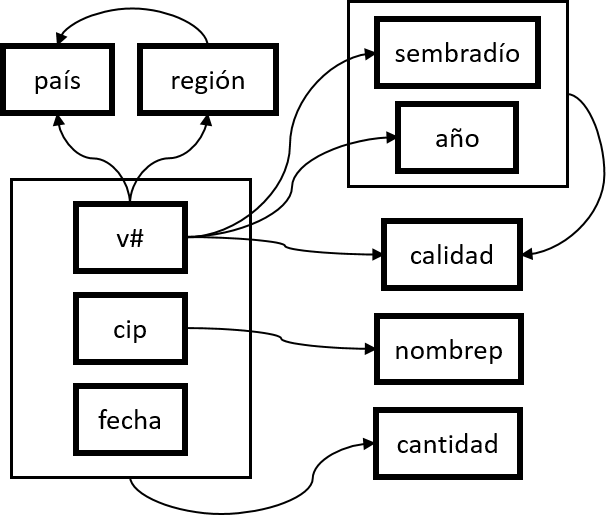
\includegraphics[scale=0.7]{img/1_1nf.png}
	\caption{1era Forma Normal}
\end{figure}

\newpage
\subsection*{2NF}
Tenemos que sembradio, año, calidad, región, país, y nombrep no dependen totalmente de la clave primaria, por lo que procedemos a separar la relación, y tendríamos:

Almacen(\underline{v\#}, \underline{cip}, \underline{fecha}, cantidad)

Produccion(\underline{v\#}, sembradio, año, calidad, region, pais)

Nombres(\underline{cip}, nombrep)

\begin{figure}[H]
	\centering
	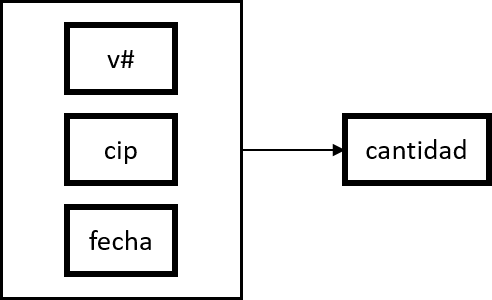
\includegraphics[scale=0.52]{img/2nf_almacen.png} 
	\hspace{0.4cm} \vrule \hspace{0.4cm}
	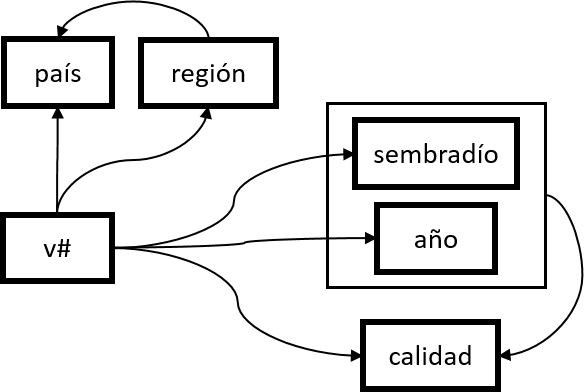
\includegraphics[scale=0.52]{img/2nf_produccion.png}
	\hspace{0.4cm} \vrule \hspace{0.4cm}
	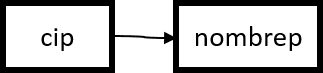
\includegraphics[scale=0.52]{img/2nf_nombres.png}
	\caption{Almacen, Produccion y Nombres}
\end{figure}


\subsection*{3NF}
Tenemos que calidad y pais no dependen solo de la clave primaria, por lo que:

Almacen(\underline{v\#}, \underline{cip}, \underline{fecha}, cantidad)

Produccion(\underline{v\#}, sembradio, año, región)

Siembras(\underline{sembradio}, \underline{año}, calidad)

Lugares(\underline{región}, país)

Nombres(\underline{cip}, nombrep)

